\documentclass[12pt,a4paper]{report}

% ==================== PACKAGES ====================
\usepackage[utf8]{inputenc}
\usepackage[T1]{fontenc}
\usepackage{graphicx}
\usepackage{geometry}
\usepackage{titlesec}
\usepackage{fancyhdr}
\usepackage{booktabs}
\usepackage{longtable}
\usepackage{array}
\usepackage{multirow}
\usepackage{xcolor}
\usepackage{listings}
\usepackage{hyperref}
\usepackage{caption}
\usepackage{float}
\usepackage{enumitem}
\usepackage{tocloft}
\usepackage{parskip}
\usepackage{setspace}

% ==================== PAGE GEOMETRY ====================
\geometry{
    top=1in,
    bottom=1in,
    left=1.25in,
    right=1in
}

% ==================== COLORS ====================
\definecolor{ioeblue}{RGB}{0, 51, 102}
\definecolor{codegray}{RGB}{245, 245, 245}
\definecolor{codegreen}{RGB}{0, 128, 0}

% ==================== HYPERREF SETUP ====================
\hypersetup{
    colorlinks=true,
    linkcolor=ioeblue,
    filecolor=magenta,
    urlcolor=blue,
    citecolor=ioeblue
}

% ==================== LISTINGS SETUP ====================
\lstset{
    backgroundcolor=\color{codegray},
    basicstyle=\ttfamily\small,
    breaklines=true,
    captionpos=b,
    keepspaces=true,
    numbers=left,
    numbersep=5pt,
    numberstyle=\tiny\color{gray},
    showspaces=false,
    showstringspaces=false,
    frame=single,
    rulecolor=\color{gray},
    keywordstyle=\color{ioeblue}\bfseries,
    commentstyle=\color{codegreen},
    stringstyle=\color{red}
}

% ==================== HEADER/FOOTER ====================
\pagestyle{fancy}
\fancyhf{}
\fancyhead[L]{\small\leftmark}
\fancyhead[R]{\small CT 654 -- Computer Networks}
\fancyfoot[C]{\thepage}
\renewcommand{\headrulewidth}{0.4pt}
\renewcommand{\footrulewidth}{0.4pt}

% ==================== CHAPTER FORMATTING (no "Chapter X" prefix) ====================
\titleformat{\chapter}[display]
{\normalfont\Huge\bfseries\color{ioeblue}}
{}{0pt}{}
\titlespacing*{\chapter}{0pt}{-30pt}{20pt}

% ==================== BEGIN DOCUMENT ====================
\begin{document}

% ==================== COVER PAGE ====================
\begin{titlepage}
    \centering
    \vspace*{0.5cm}
    
    % Emblem
    
\includegraphics[width=0.25\textwidth]{emblem.png}
    
    \vspace{0.5cm}
    
    {\Large\bfseries TRIBHUVAN UNIVERSITY}\\[0.3cm]
    {\large INSTITUTE OF ENGINEERING}\\[0.2cm]
    {\large PULCHOWK CAMPUS}\\[0.2cm]
    {\normalsize Department of Electronics and Computer Engineering}
    
    \vspace{1.5cm}
    
    \rule{\textwidth}{1.5pt}\\[0.4cm]
    {\Huge\bfseries\color{ioeblue} Network Design and Implementation\\[0.2cm] for Fishtail Hospital}\\[0.3cm]
    \rule{\textwidth}{1.5pt}
    
    \vspace{2cm}
    
    \begin{minipage}[t]{0.45\textwidth}
        \centering
        \textbf{Submitted By:}\\[0.3cm]
        \large Chandan Kumar Shah\\
        Roll No: 080BCT023\\
        B.E. Computer Engineering
    \end{minipage}
    \hfill
    \begin{minipage}[t]{0.45\textwidth}
        \centering
        \textbf{Submitted To:}\\[0.3cm]
        \large Department of Electronics\\and Computer Engineering\\
        Pulchowk Campus, IOE
    \end{minipage}
    
    \vfill
    
    {\large April 2026}
    
\end{titlepage}

% ==================== TABLE OF CONTENTS ====================
\pagenumbering{roman}
\tableofcontents
\newpage
\listoffigures
\newpage
\listoftables
\newpage

% ==================== MAIN CONTENT ====================
\pagenumbering{arabic}

% ==================== ABSTRACT ====================
\chapter*{Abstract}
\addcontentsline{toc}{chapter}{Abstract}

This report presents the design and implementation of a comprehensive network infrastructure for Fishtail Hospital, a multi-department healthcare facility. The network employs a hierarchical topology with 10 routers, 5 switches, and 28 total devices, utilizing OSPF multi-area routing across three areas for efficient traffic management. Variable Length Subnet Masking (VLSM) is implemented to optimize IP address allocation from the assigned 172.16.0.0/22 block, achieving approximately 60\% utilization. Seven VLANs provide department-level segmentation, with essential network services including DNS, DHCP, and web servers deployed across the infrastructure. All project requirements have been successfully met, demonstrating practical application of computer networking concepts in a realistic healthcare scenario.

\newpage

% ==================== CHAPTER 1: INTRODUCTION ====================
\chapter{Introduction}

\section{Background}
Modern healthcare facilities require robust and reliable network infrastructure to support critical operations including patient records management, diagnostic systems, administrative functions, and communication services. The Fishtail Hospital network project addresses these requirements through a comprehensive network design that ensures connectivity, security, and scalability.

\section{Project Objectives}
The primary objectives of this project are:
\begin{itemize}[noitemsep]
    \item Design and implement a multi-department hospital network using Cisco networking equipment
    \item Implement efficient IP addressing using VLSM (Variable Length Subnet Masking)
    \item Configure OSPF multi-area routing for optimal traffic management
    \item Deploy VLAN segmentation for department isolation and security
    \item Establish essential network services including DNS, DHCP, and Web servers
    \item Implement router security measures for controlled access
\end{itemize}

\section{Project Scope}
\begin{table}[H]
\centering
\caption{Project Scope Summary}
\begin{tabular}{ll}
\toprule
\textbf{Parameter} & \textbf{Value} \\
\midrule
Course & CT 654 -- Computer Networks \\
Institution & IOE, Pulchowk Campus, Tribhuvan University \\
Tool Used & Cisco Packet Tracer 8.x \\
IP Block Assigned & 172.16.0.0/22 (1024 addresses) \\
Scenario & Multi-department hospital with ISP connectivity \\
\bottomrule
\end{tabular}
\end{table}

% ==================== CHAPTER 2: REQUIREMENTS ANALYSIS ====================
\chapter{Requirements Analysis}

\section{Project Requirements Checklist}
Table \ref{tab:requirements} presents the complete list of project requirements and their fulfillment status.

\begin{table}[H]
\centering
\caption{Requirements Verification Matrix}
\label{tab:requirements}
\begin{tabular}{p{7cm}cc}
\toprule
\textbf{Requirement} & \textbf{Status} & \textbf{Implementation Detail} \\
\midrule
Minimum 10 routers & \checkmark & 10 routers (ISP-R1 + Chandan1--9) \\
At least 3 transit routers & \checkmark & Chandan4, Chandan5, Chandan8 \\
ISP router + connection & \checkmark & ISP-R1 with 203.0.113.0/24 \\
At least 9 LANs with 6 subnet sizes & \checkmark & 9 LANs + 9 P2P links \\
OSPF multi-area (minimum 3 areas) & \checkmark & Area 0, Area 1, Area 2 \\
Minimum 7 VLANs & \checkmark & VLAN 10, 20, 30, 40, 50, 60, 70 \\
At least 2 VLANs spanning 3+ switches & \checkmark & VLAN 10 \& 20 (SW3/SW4/SW5) \\
Minimum 3 DNS servers & \checkmark & DNS1, DNS2, ISP-DNS \\
Minimum 2 Web servers & \checkmark & WebServer1, WebServer2 \\
Minimum 3 DHCP servers & \checkmark & DHCP1, DHCP2, DHCP3 \\
Router security (passwords + telnet) & \checkmark & All 9 routers configured \\
Router naming convention & \checkmark & Chandan1--Chandan9 \\
VLSM addressing & \checkmark & 6 different prefix lengths \\
Interface labeling & \checkmark & All IPs labeled in topology \\
\bottomrule
\end{tabular}
\end{table}

\section{Device Inventory}
\begin{table}[H]
\centering
\caption{Network Device Inventory}
\label{tab:inventory}
\begin{tabular}{llcl}
\toprule
\textbf{Device Type} & \textbf{Model} & \textbf{Qty} & \textbf{Role} \\
\midrule
Routers & Cisco 2911 & 10 & ISP-R1 + Chandan1--9 \\
Switches & Cisco 2960-24TT & 5 & SW1, SW2, SW3, SW4, SW5 \\
Servers & Server-PT & 8 & DNS, DHCP, Web, ISP \\
Workstations & PC-PT & 5 & Admin, OPD, Ward, ICU \\
\midrule
\textbf{TOTAL} & & \textbf{28} & \\
\bottomrule
\end{tabular}
\end{table}

% ==================== CHAPTER 3: NETWORK DESIGN ====================
\chapter{Network Design}

\section{Network Topology}
The network follows a hierarchical design with clear separation between core, distribution, and access layers. Figure \ref{fig:topology} illustrates the complete network topology.

\begin{figure}[H]
\centering
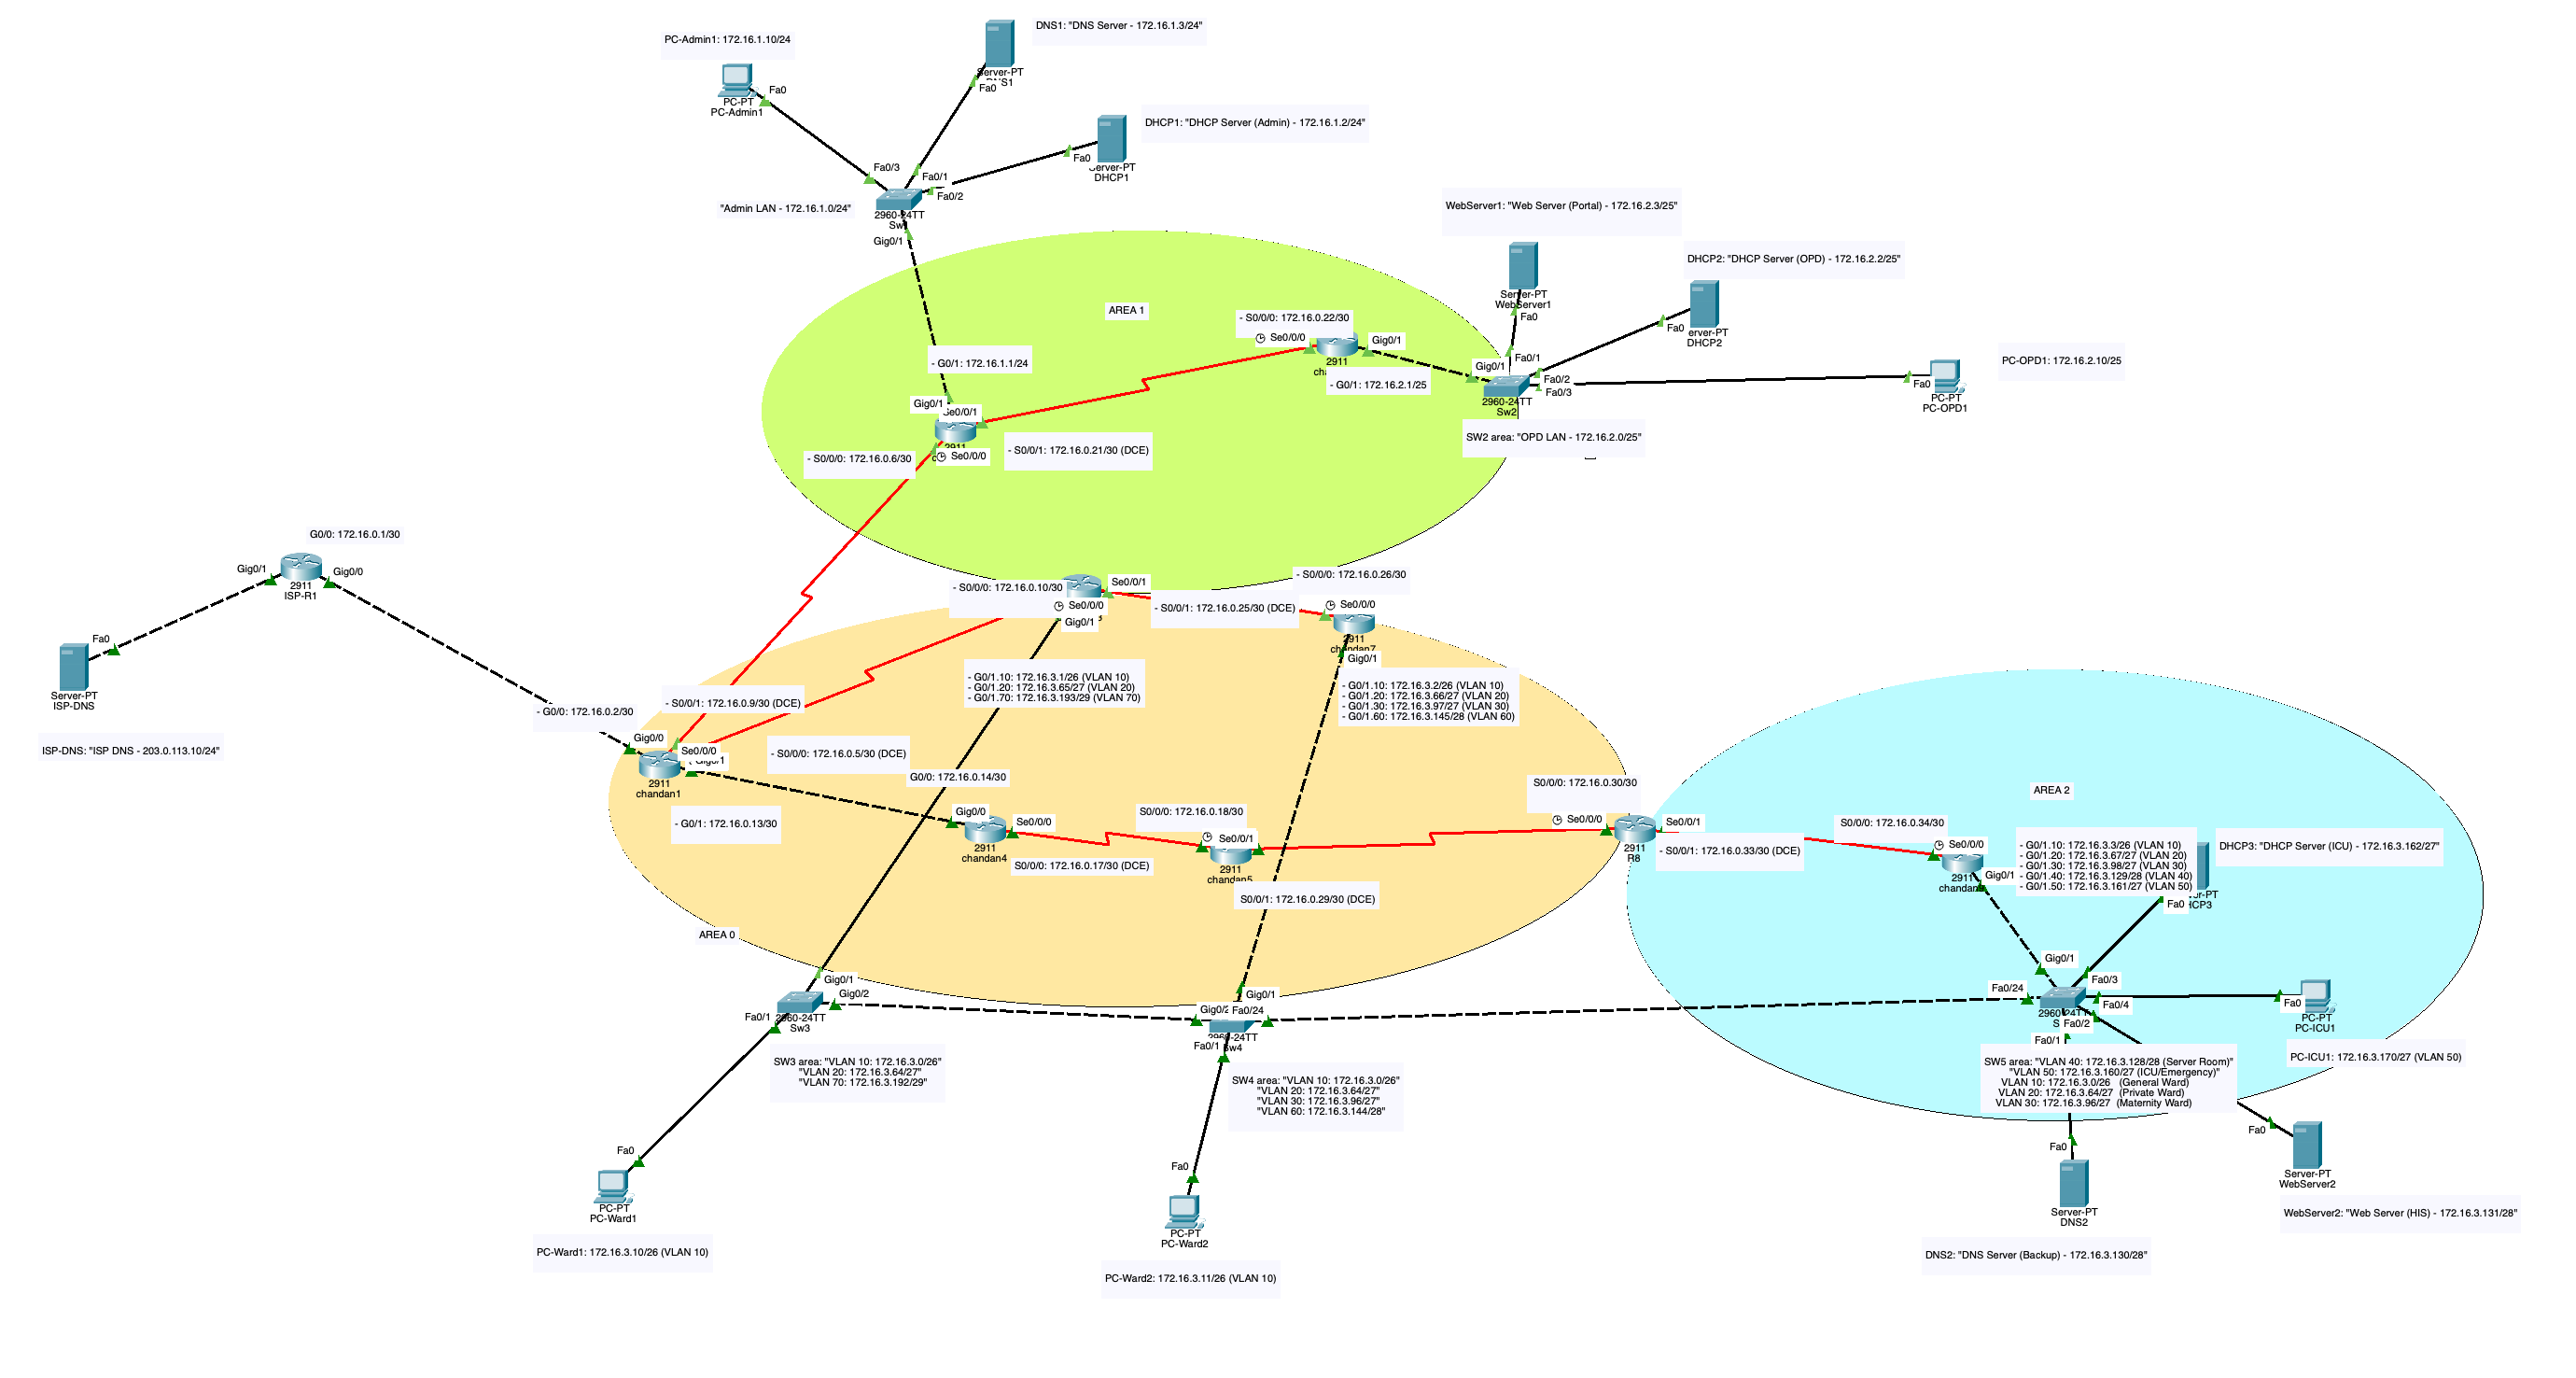
\includegraphics[width=\textwidth]{topology.png}
\caption{Fishtail Hospital Network Topology}
\label{fig:topology}
\end{figure}

\section{Topology Structure}
The network architecture consists of:
\begin{itemize}[noitemsep]
    \item \textbf{ISP-R1}: External gateway providing internet connectivity
    \item \textbf{Chandan1}: Core router and ASBR (Autonomous System Boundary Router)
    \item \textbf{Chandan3, Chandan8}: Area Border Routers (ABRs)
    \item \textbf{Chandan4, Chandan5}: Transit routers for backbone connectivity
    \item \textbf{Chandan2, Chandan6, Chandan7, Chandan9}: Access layer routers
\end{itemize}

\section{OSPF Multi-Area Design}
Open Shortest Path First (OSPF) protocol is implemented with three areas for optimal routing performance.

\begin{table}[H]
\centering
\caption{OSPF Area Assignment}
\label{tab:ospf}
\begin{tabular}{p{3.5cm}p{6.5cm}p{4cm}}
\toprule
\textbf{OSPF Area} & \textbf{Routers} & \textbf{Type} \\
\midrule
Area 0 (Backbone) & Chandan1, Chandan3, Chandan4, Chandan5, Chandan8 & Transit/Core \\
Area 1 & Chandan2, Chandan3, Chandan6, Chandan7 & Admin/OPD/Ward \\
Area 2 & Chandan8, Chandan9 & ICU/Server Room \\
\bottomrule
\end{tabular}
\end{table}

\subsection{Router Roles}
\begin{itemize}[noitemsep]
    \item \textbf{ABR (Area Border Routers):}
    \begin{itemize}
        \item Chandan3 -- boundary of Area 0 and Area 1
        \item Chandan8 -- boundary of Area 0 and Area 2
    \end{itemize}
    \item \textbf{ASBR (Autonomous System Boundary Router):}
    \begin{itemize}
        \item Chandan1 -- redistributes static default route from ISP into OSPF
    \end{itemize}
\end{itemize}

% ==================== CHAPTER 4: IP ADDRESSING ====================
\chapter{IP Addressing Scheme}

\section{VLSM Implementation}
Variable Length Subnet Masking (VLSM) is employed to efficiently utilize the assigned IP block 172.16.0.0/22, providing 1024 total addresses.

\section{Point-to-Point Links}
All router interconnections use /30 subnets, providing 2 usable host addresses per link.

\begin{table}[H]
\centering
\caption{Point-to-Point Link Addressing}
\label{tab:p2p}
\begin{tabular}{llll}
\toprule
\textbf{Link} & \textbf{Network} & \textbf{Router A IP} & \textbf{Router B IP} \\
\midrule
ISP-R1 $\leftrightarrow$ Chandan1 & 172.16.0.0/30 & 172.16.0.1 & 172.16.0.2 \\
Chandan1 $\leftrightarrow$ Chandan2 & 172.16.0.4/30 & 172.16.0.5 & 172.16.0.6 \\
Chandan1 $\leftrightarrow$ Chandan3 & 172.16.0.8/30 & 172.16.0.9 & 172.16.0.10 \\
Chandan1 $\leftrightarrow$ Chandan4 & 172.16.0.12/30 & 172.16.0.13 & 172.16.0.14 \\
Chandan4 $\leftrightarrow$ Chandan5 & 172.16.0.16/30 & 172.16.0.17 & 172.16.0.18 \\
Chandan2 $\leftrightarrow$ Chandan6 & 172.16.0.20/30 & 172.16.0.21 & 172.16.0.22 \\
Chandan3 $\leftrightarrow$ Chandan7 & 172.16.0.24/30 & 172.16.0.25 & 172.16.0.26 \\
Chandan5 $\leftrightarrow$ Chandan8 & 172.16.0.28/30 & 172.16.0.29 & 172.16.0.30 \\
Chandan8 $\leftrightarrow$ Chandan9 & 172.16.0.32/30 & 172.16.0.33 & 172.16.0.34 \\
\bottomrule
\end{tabular}
\end{table}

\section{LAN Subnets}
Six different prefix lengths are used to accommodate varying department sizes.

\begin{table}[H]
\centering
\caption{LAN Subnet Allocation}
\label{tab:lan}
\begin{tabular}{lclccc}
\toprule
\textbf{Department} & \textbf{VLAN} & \textbf{Subnet} & \textbf{Gateway} & \textbf{Hosts} & \textbf{Prefix} \\
\midrule
Administration & -- & 172.16.1.0/24 & 172.16.1.1 & 254 & /24 \\
OPD & -- & 172.16.2.0/25 & 172.16.2.1 & 126 & /25 \\
General Ward & 10 & 172.16.3.0/26 & 172.16.3.1 & 62 & /26 \\
Private Ward & 20 & 172.16.3.64/27 & 172.16.3.65 & 30 & /27 \\
Maternity Ward & 30 & 172.16.3.96/27 & 172.16.3.97 & 30 & /27 \\
Server Room & 40 & 172.16.3.128/28 & 172.16.3.129 & 14 & /28 \\
Laboratory & 60 & 172.16.3.144/28 & 172.16.3.145 & 14 & /28 \\
ICU / Emergency & 50 & 172.16.3.160/27 & 172.16.3.161 & 30 & /27 \\
Pharmacy & 70 & 172.16.3.192/29 & 172.16.3.193 & 6 & /29 \\
ISP Public & -- & 203.0.113.0/24 & 203.0.113.1 & 254 & /24 \\
\bottomrule
\end{tabular}
\end{table}

\section{Address Utilization}
\begin{table}[H]
\centering
\caption{IP Address Utilization Summary}
\begin{tabular}{lr}
\toprule
\textbf{Category} & \textbf{Addresses} \\
\midrule
P2P links (9 $\times$ /30) & 36 \\
Admin LAN (/24) & 254 \\
OPD LAN (/25) & 126 \\
VLAN subnets combined & 196 \\
\midrule
\textbf{Total Used} & \textbf{$\sim$612} \\
Reserved for expansion & $\sim$412 \\
\textbf{Total Block} & \textbf{1024} \\
\bottomrule
\end{tabular}
\end{table}

% ==================== CHAPTER 5: VLAN CONFIGURATION ====================
\chapter{VLAN Configuration}

\section{VLAN Design}
Seven VLANs are configured to segment network traffic by department and function.

\begin{table}[H]
\centering
\caption{VLAN Configuration}
\label{tab:vlan}
\begin{tabular}{clll}
\toprule
\textbf{VLAN ID} & \textbf{Name} & \textbf{Subnet} & \textbf{Switch Coverage} \\
\midrule
10 & General-Ward & 172.16.3.0/26 & SW3 + SW4 + SW5 \\
20 & Private-Ward & 172.16.3.64/27 & SW3 + SW4 + SW5 \\
30 & Maternity-Ward & 172.16.3.96/27 & SW4 + SW5 \\
40 & Server-Room & 172.16.3.128/28 & SW5 \\
50 & ICU-Emergency & 172.16.3.160/27 & SW5 \\
60 & Laboratory & 172.16.3.144/28 & SW4 \\
70 & Pharmacy & 172.16.3.192/29 & SW3 \\
\bottomrule
\end{tabular}
\end{table}

\textbf{Note:} VLAN 10 and VLAN 20 span 3 switches (SW3 $\rightarrow$ SW4 $\rightarrow$ SW5) via 802.1Q trunk links.

\section{Trunk Links}
\begin{itemize}[noitemsep]
    \item SW3 Gig0/2 $\leftrightarrow$ SW4 Gig0/2 (trunk)
    \item SW4 Fa0/24 $\leftrightarrow$ SW5 Fa0/24 (trunk)
\end{itemize}

\section{Inter-VLAN Routing}
Router-on-a-stick method using 802.1Q subinterfaces:

\begin{table}[H]
\centering
\caption{Inter-VLAN Routing Configuration}
\begin{tabular}{lll}
\toprule
\textbf{Router} & \textbf{Handles VLANs} & \textbf{Connected Switch} \\
\midrule
Chandan3 & VLAN 10, 20, 70 & SW3 \\
Chandan7 & VLAN 10, 20, 30, 60 & SW4 \\
Chandan9 & VLAN 10, 20, 30, 40, 50 & SW5 \\
\bottomrule
\end{tabular}
\end{table}

% ==================== CHAPTER 6: NETWORK SERVICES ====================
\chapter{Network Services}

\section{DNS Servers}
Three DNS servers provide name resolution services across the network.

\begin{table}[H]
\centering
\caption{DNS Server Configuration}
\begin{tabular}{llll}
\toprule
\textbf{Server} & \textbf{IP Address} & \textbf{Location} & \textbf{Role} \\
\midrule
DNS1 & 172.16.1.3 & Admin LAN/SW1 & Primary -- resolves hospital.local \\
DNS2 & 172.16.3.130 & Server Room/SW5 & Backup DNS \\
ISP-DNS & 203.0.113.10 & ISP Network & External/Internet DNS \\
\bottomrule
\end{tabular}
\end{table}

\textbf{DNS Record:} \texttt{hospital.local $\rightarrow$ 172.16.2.3 (WebServer1)}

\section{DHCP Servers}
Three DHCP servers provide automatic IP configuration for different network zones.

\begin{table}[H]
\centering
\caption{DHCP Server Configuration}
\begin{tabular}{lllll}
\toprule
\textbf{Server} & \textbf{IP Address} & \textbf{Pool Range} & \textbf{Gateway} & \textbf{Serves} \\
\midrule
DHCP1 & 172.16.1.2 & 172.16.1.20--119 & 172.16.1.1 & Admin LAN \\
DHCP2 & 172.16.2.2 & 172.16.2.20--69 & 172.16.2.1 & OPD LAN \\
DHCP3 & 172.16.3.162 & 172.16.3.175--190 & 172.16.3.161 & ICU (VLAN 50) \\
\bottomrule
\end{tabular}
\end{table}

\section{Web Servers}
\begin{table}[H]
\centering
\caption{Web Server Configuration}
\begin{tabular}{llll}
\toprule
\textbf{Server} & \textbf{IP Address} & \textbf{URL} & \textbf{Purpose} \\
\midrule
WebServer1 & 172.16.2.3 & http://hospital.local & Public Hospital Portal \\
WebServer2 & 172.16.3.131 & -- & Hospital Information System \\
\bottomrule
\end{tabular}
\end{table}

% ==================== CHAPTER 7: ROUTER CONFIGURATION ====================
\chapter{Router Configuration}

\section{Interface Configuration Example -- Chandan1}
\begin{lstlisting}[caption={Chandan1 Interface Configuration},language=bash]
hostname Chandan1
interface GigabitEthernet0/0
 ip address 172.16.0.2 255.255.255.252
 no shutdown
interface GigabitEthernet0/1
 ip address 172.16.0.13 255.255.255.252
 no shutdown
interface Serial0/0/0
 ip address 172.16.0.5 255.255.255.252
 clock rate 64000
 no shutdown
interface Serial0/0/1
 ip address 172.16.0.9 255.255.255.252
 clock rate 64000
 no shutdown
ip route 0.0.0.0 0.0.0.0 172.16.0.1
\end{lstlisting}

\section{Router-on-a-Stick Configuration -- Chandan3}
\begin{lstlisting}[caption={Chandan3 Subinterface Configuration},language=bash]
interface GigabitEthernet0/1
 no shutdown
interface GigabitEthernet0/1.10
 encapsulation dot1Q 10
 ip address 172.16.3.1 255.255.255.192
interface GigabitEthernet0/1.20
 encapsulation dot1Q 20
 ip address 172.16.3.65 255.255.255.224
interface GigabitEthernet0/1.70
 encapsulation dot1Q 70
 ip address 172.16.3.193 255.255.255.248
\end{lstlisting}

\section{OSPF Configuration -- Chandan1}
\begin{lstlisting}[caption={Chandan1 OSPF Configuration},language=bash]
router ospf 1
 router-id 1.1.1.1
 network 172.16.0.0 0.0.0.3 area 0
 network 172.16.0.4 0.0.0.3 area 1
 network 172.16.0.8 0.0.0.3 area 1
 network 172.16.0.12 0.0.0.3 area 0
 default-information originate
\end{lstlisting}

% ==================== CHAPTER 8: SECURITY CONFIGURATION ====================
\chapter{Security Configuration}

\section{Router Security Settings}
Security measures applied to all routers (Chandan1 through Chandan9):

\begin{table}[H]
\centering
\caption{Security Configuration Summary}
\begin{tabular}{ll}
\toprule
\textbf{Security Feature} & \textbf{Value} \\
\midrule
Console password & cisco \\
Enable secret & class \\
VTY (Telnet) password & network \\
Password encryption & service password-encryption enabled \\
Telnet access & line vty 0 4, transport input telnet \\
\bottomrule
\end{tabular}
\end{table}

\section{Security Configuration Commands}
\begin{lstlisting}[caption={Security Configuration for All Routers},language=bash]
enable secret class
service password-encryption
line console 0
 password cisco
 login
line vty 0 4
 password network
 login
 transport input telnet
\end{lstlisting}

\textbf{Telnet Test:} From PC-Admin1 $\rightarrow$ \texttt{telnet 172.16.1.1} $\rightarrow$ login: \texttt{network} $\rightarrow$ enable: \texttt{class}

% ==================== CHAPTER 9: TESTING AND VERIFICATION ====================
\chapter{Testing and Verification}

\section{Connectivity Test Results}
All tests were conducted from PC-Admin1 (172.16.1.10):

\begin{table}[H]
\centering
\caption{Network Connectivity Test Results}
\begin{tabular}{llcc}
\toprule
\textbf{Test} & \textbf{Destination} & \textbf{Result} & \textbf{Packet Loss} \\
\midrule
Gateway reachability & 172.16.1.1 & PASS & 0\% \\
Cross-area (OSPF IA) & 172.16.2.10 & PASS & 25\% (1st ARP) \\
Cross-VLAN (Ward) & 172.16.3.10 & PASS & 25\% (1st) \\
Cross-area to ICU & 172.16.3.170 & PASS & 25\% (1st) \\
To ISP (static route) & 203.0.113.10 & PASS & 50\% (1st 2) \\
DNS resolution & hospital.local & PASS & Resolved \\
\bottomrule
\end{tabular}
\end{table}

\textbf{Note:} First-packet loss is expected in Packet Tracer due to ARP resolution and OSPF convergence delays. After convergence, 0\% loss is observed.

\section{OSPF Verification}
OSPF verification on Chandan1 shows:
\begin{itemize}[noitemsep]
    \item Routes marked \texttt{O} = intra-area OSPF
    \item Routes marked \texttt{O IA} = inter-area OSPF
    \item Route marked \texttt{S*} = default static route to ISP
\end{itemize}

% ==================== CHAPTER 10: DESIGN RATIONALE ====================
\chapter{Design Rationale}

\section{Why VLSM?}
The 172.16.0.0/22 block provides 1024 addresses. Different departments have vastly different size requirements -- Administration needs 254 hosts while Pharmacy needs only 6. VLSM prevents IP address wastage by assigning exactly the prefix length needed for each subnet.

\section{Why OSPF Multi-Area?}
A single flat OSPF area would flood Link State Advertisements (LSAs) to every router, wasting bandwidth and processing power. Splitting into 3 areas (Area 0 backbone + 2 stub areas) contains LSA flooding within each area. Only summarized routes cross area boundaries, improving scalability.

\section{Why Router-on-a-Stick?}
Only one physical cable runs from each router to its switch, but using 802.1Q subinterfaces, multiple VLANs are carried over that single link. Each subinterface acts as a separate gateway for its respective VLAN, providing cost-effective inter-VLAN routing.

\section{Why VLANs Spanning Multiple Switches?}
General Ward (VLAN 10) and Private Ward (VLAN 20) patients are spread across multiple floors. The same VLAN allows seamless mobility -- a laptop moving from Floor 1 (SW3) to Floor 2 (SW4) or Server Room (SW5) maintains the same IP subnet without reconfiguration.

\section{Why Multiple DHCP Servers?}
Each major zone (Admin, OPD, ICU) has its own local DHCP server to reduce cross-network DHCP traffic and provide redundancy. The \texttt{ip helper-address} command relays DHCP requests from subnets without a local server.

\section{Serial vs GigabitEthernet Links}
Serial links simulate WAN connections between distant building floors or wings, representing realistic bandwidth constraints. GigabitEthernet is used for high-speed campus backbone links (ISP-R1$\leftrightarrow$Chandan1, Chandan1$\leftrightarrow$Chandan4) where high throughput is required.

% ==================== CHAPTER 11: PROJECT STATISTICS ====================
\chapter{Project Statistics}

\begin{table}[H]
\centering
\caption{Complete Project Statistics}
\begin{tabular}{lr}
\toprule
\textbf{Metric} & \textbf{Value} \\
\midrule
Total routers & 10 \\
Transit-only routers & 3 (Chandan4, 5, 8) \\
Area Border Routers (ABRs) & 2 (Chandan3, Chandan8) \\
AS Boundary Router (ASBR) & 1 (Chandan1) \\
Total switches & 5 \\
Total servers & 8 \\
Total workstations & 5 \\
\textbf{Total devices} & \textbf{28} \\
\midrule
OSPF areas & 3 \\
VLANs configured & 7 \\
VLANs spanning 3 switches & 2 (VLAN 10, 20) \\
P2P subnets (/30) & 9 \\
LAN subnets & 9 (+1 ISP) \\
Different prefix lengths & 6 \\
\midrule
DNS servers & 3 \\
DHCP servers & 3 \\
Web servers & 2 \\
\midrule
Total IP addresses in block & 1024 \\
Addresses actually used & $\sim$612 \\
\bottomrule
\end{tabular}
\end{table}

% ==================== CHAPTER 12: CONCLUSION ====================
\chapter{Conclusion}

The Fishtail Hospital network design project successfully demonstrates the implementation of a comprehensive enterprise network infrastructure. All project requirements have been met, including:

\begin{itemize}[noitemsep]
    \item Deployment of 10 routers with proper naming convention (Chandan1--Chandan9 + ISP-R1)
    \item Implementation of OSPF multi-area routing with 3 areas for optimal traffic management
    \item Configuration of 7 VLANs with 2 VLANs spanning 3 switches for department segmentation
    \item Efficient IP address utilization through VLSM with 6 different prefix lengths
    \item Establishment of essential network services (DNS, DHCP, Web) for hospital operations
    \item Implementation of router security measures for controlled network access
\end{itemize}

The network design demonstrates practical application of computer networking concepts including subnetting, routing protocols, VLAN segmentation, and network services. The hierarchical topology ensures scalability for future expansion while the current implementation efficiently utilizes approximately 60\% of the allocated IP address space.

\vspace{1cm}
\begin{center}
\rule{0.4\textwidth}{0.4pt}
\end{center}

\end{document}
